\chapter{E-puck2 Demos}
\label{chap:demos}
\shorttitle{\nameref{chap:demos}}

Once a robot has running \ac{ros2} driver, \ac{ros2} nodes can be built on top of it, or community \ac{ros2} nodes can be integrated.
Therefore, in this chapter, various examples that utilize the e-puck2's \ac{ros2} interface will be shown while focusing on custom-built nodes.
All demos presented in this chapter work with both the physical and simulated e-puck2 robots.
Some demos are also successfully tested with a few other simulated robots.

\section{Visualizations}
\acs{rviz2} acts as a \ac{ros2} node, and it allows users to visualize the robot's state and robot's perception of the environment in 3D.
This tool is officially supported and developed by the \ac{ros2} team; it is commonly used in \ac{ros2} applications for visualizations and is extensively utilized throughout this project. 
Therefore, a few use-cases will be given here.

\begin{figure}[H]
    \centering
    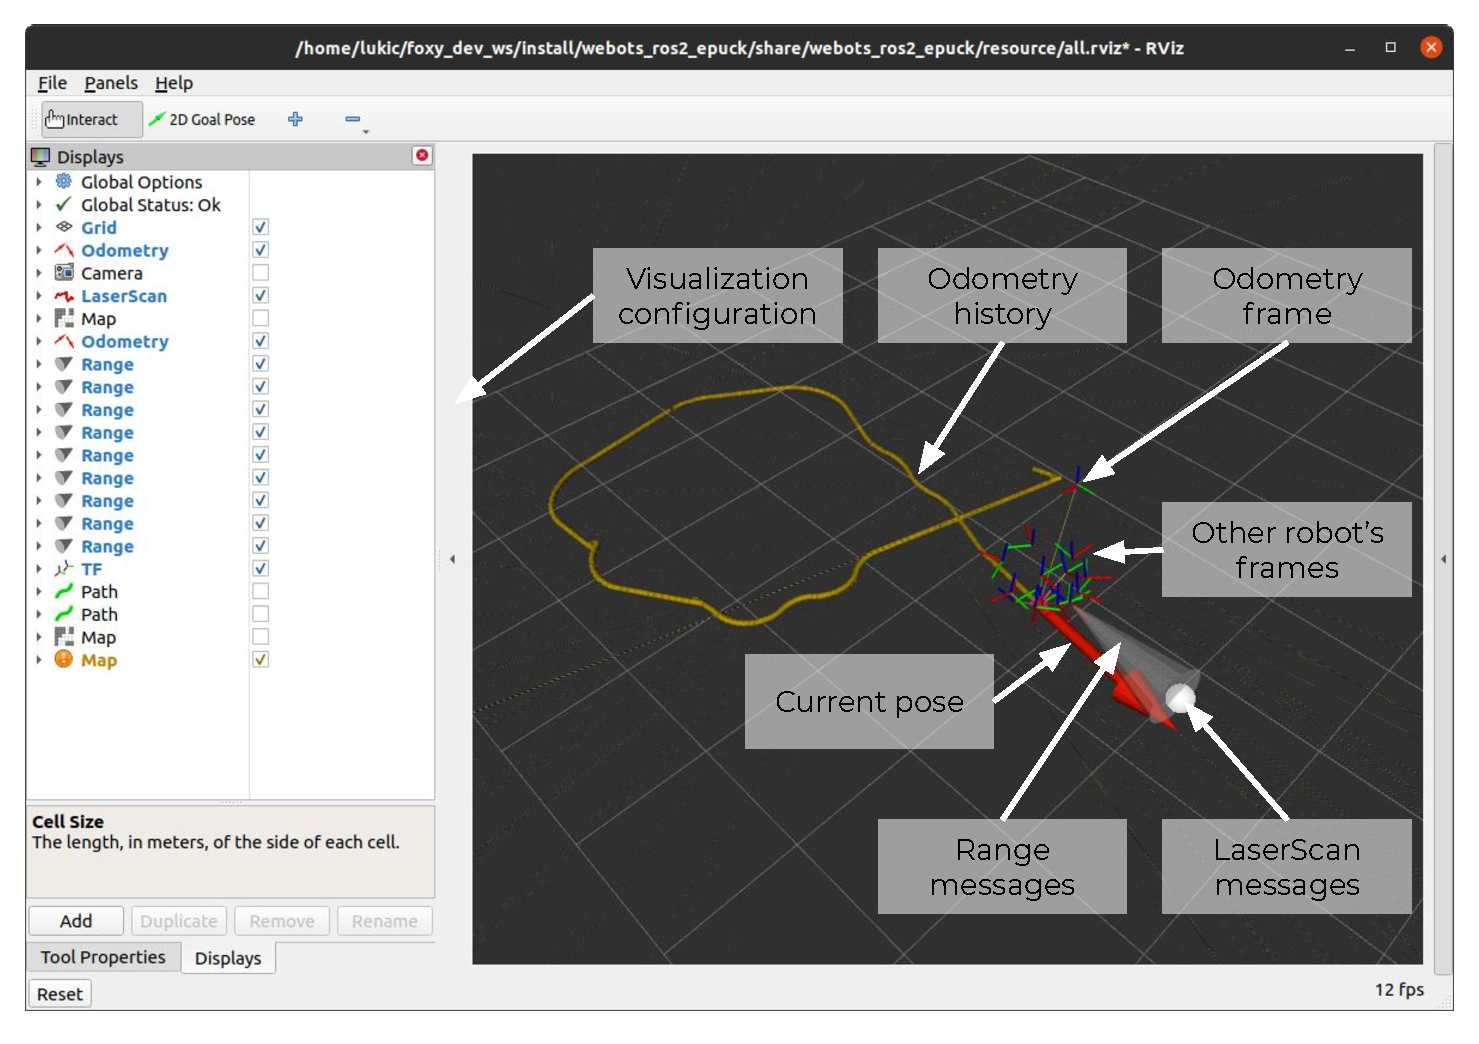
\includegraphics[width=\textwidth]{demos/figures/rviz.pdf}
    \caption{Typical visualization of e-puck2 in \acs{rviz2}}
    \label{fig:demos:rviz}
\end{figure}

\ac{rviz2} is very customizable, meaning it can visualize different aspects of the robot depending on the user's needs.
Once the user is satisfied with the visualization, the view can be saved to a file, for later reuse.
In this master project, there are many \ac{rviz2} configurations provided, optimized for different scenarios like sensor inspection, mapping, and navigation.
These configurations will be automatically loaded, depending on the launch file that is used.

In Figure \ref{fig:demos:rviz} a default view of \acs{rviz2} for the e-puck2 robot is shown.
It visualizes the robot's pose obtained from the odometry, history of odometry readings, different coordinate systems (like odometry, robot's base, distance sensors and similar), range, and laser scan measurements.

\section{Drive Calibration}

Two constants are essential in order to have accurate odometry: wheelbase (distance between the contact points of the two wheels), and wheel radius.
These constants can be measured, but even with the perfect measurements, they are subject to systematic odometry errors, caused by imperfections in the design and mechanical implementation of a mobile robot.
Typical systematic error is uncertainty about the wheelbase and means that the rubber tires contact the floor not in one point, but rather in a contact area \cite{borenstein_measurement_1996}.

Therefore, we use \texttt{/odom} and \texttt{/cmd\_vel} topics that are previously created to calibrate the two important constants for odometry.
The technique is inspired by the one presented in \cite{borenstein_measurement_1996}; the robot should move linearly, we can compare anticipated distance (self-reported distance) with the actual distance.
The linear movements allow us to adjust the wheel radius.
For the wheelbase, the robot is rotated a predefined number of rotations; then, it is compared to the actual number of rotations, and wheelbase is adjusted accordingly (see Figure \ref{fig:demos:rviz}).

\begin{figure}[H]
    \centering
    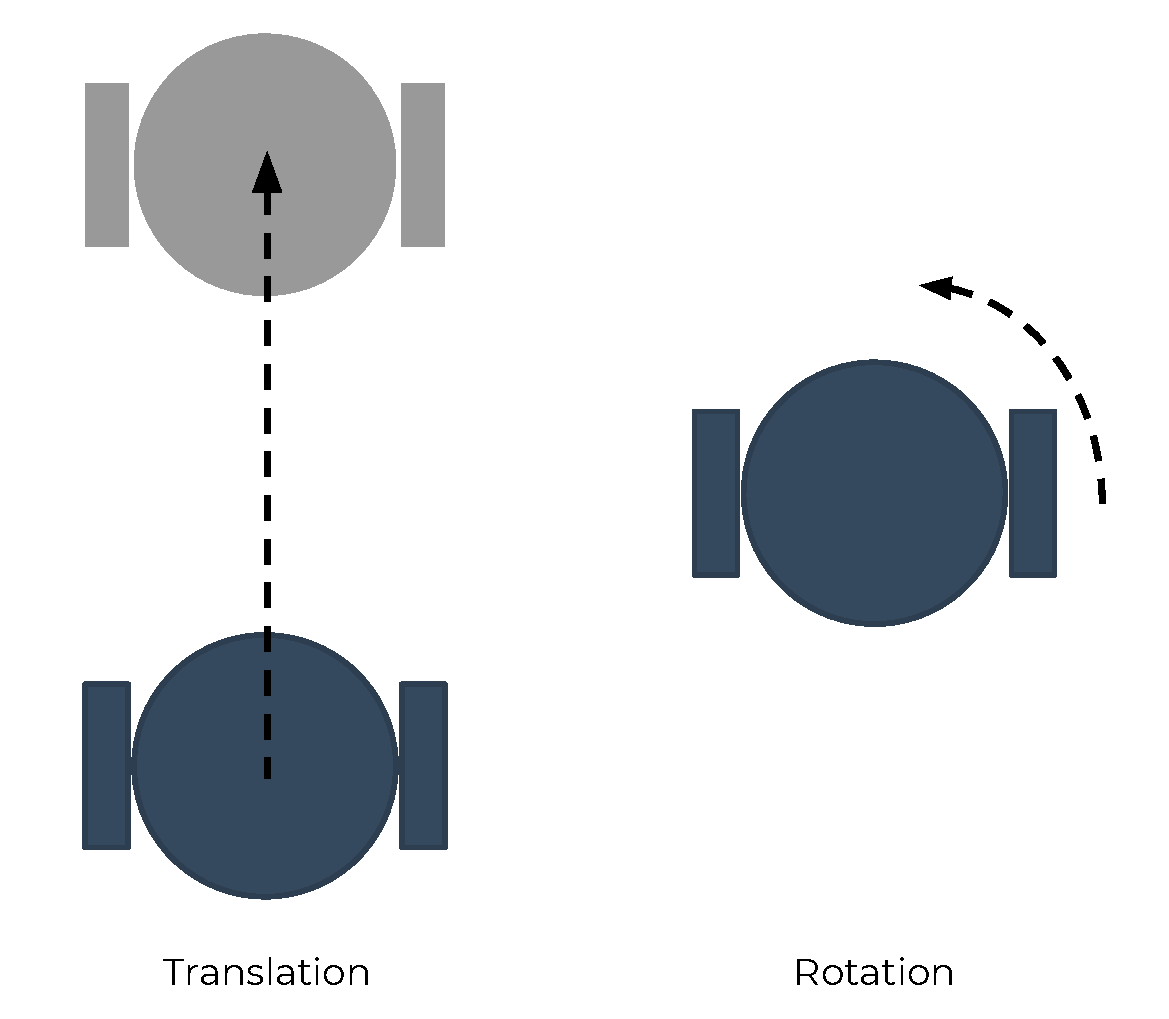
\includegraphics[width=0.7\textwidth]{demos/figures/calibration.pdf}
    \caption{Differential drive robot calibration process}
    \label{fig:demos:rviz}
\end{figure}

The custom-created node continuously receives the readings from the \texttt{/odom} topic to stop the robot exactly when the robot reaches the goal position.
It also sets appropriate linear or angular velocity depending on the type of the test.
Finally, the calibration node is successfully utilized for odometry calibration of the e-puck2 robot.
% Effectively, this node shows that \texttt{/odom} and \texttt{/cmd\_vel} topics are properly implemented while providing a useful feature.

\section{Custom Mapper Node}
\label{sec:demos:mapping}

The goal of the next example is to utilize a larger portion of the created \ac{ros2} interface.
The goal is to map the environment using an e-puck2 robot and its distance sensors.
A few approaches are considered to meet the goal:
\begin{itemize}
    \item Utilize the existing \ac{slam} solutions available for \ac{ros2} (\texttt{slam\_toolbox} or \texttt{cartographer}).
    \item Create a simple custom solution.
    \item Make a bridge to \ac{ros}1 workspace and use \ac{slam} solutions available for \ac{ros}1 (e.g. \texttt{gmapping} is only available for \ac{ros}1).
    \item Port \texttt{gmapping} \ac{slam} solution (that is available only for \ac{ros}1) to \ac{ros2}.
\end{itemize}

In tests, \texttt{slam\_toolbox} and \texttt{cartographer} were not able to provide accurate mapping due to the scarcity of the distance measurements\footnote{The author of \texttt{slam\_toolbox}, Steve Macenski, explained that modern graph-based \ac{slam} solutions do not provide good results when used with e-puck2 robot (or similar robots with a few distance sensors) like old particle filter based \ac{slam} solutions - \url{https://github.com/SteveMacenski/slam_toolbox/issues/192}.}. Using \texttt{gmapping} through \ac{ros}1 bridge indeed gave a good results.
However, complex installation and usage is something we tried to avoid as it is not user-friendly.
Porting \texttt{gmapping} to \ac{ros2} is feasible, but maintenance of a such complex software would be time intensive.

Finally, considering the scope of this master project and the high precision of e-puck2 odometry, the decision was to create a simple mapping node.
The node uses odometry exclusively for localization.
In general, this is not the right solution knowing that the odometry accumulates the error, but it provides satisfying results for small maps. 

\vspace*{.4cm}
\begin{algorithm}[H]
\SetKwInOut{Input}{input}
\SetKwInOut{Output}{output}
\Input{%
    $\bm{L_{scans}}$ -- Laser scan readings \newline 
    $\bm{P_{odom}}$ -- Position of the robot obtained from the odometry
}
\Output{%
    $\bm{M_{map}}$ -- Map of type \texttt{nav\_msgs/OccupancyGrid}
}

$ O_{world} = [\hspace{2mm}] $ \tcp{List of coordinates of obstacles}
use \texttt{tf2} to get position of laser scanner $ P_{scan} $\;

\For{each $ L_{scan} $  in $ L_{scans} $}{
    determine angle of ray ($ \alpha $) from index\;
    $ O_{x} \leftarrow P_{scan} + L_{scan} cos(\alpha) $\;
    $ O_{y} \leftarrow P_{scan} + L_{scan} sin(\alpha) $\;
    add coordinates ($O_{x}$, $O_{y}$) to $ O_{world} $\;
}

write coordinates ($O_{x}$, $O_{y}$) to $ M_{map} $\;
use Bresenham's line algorithm to write empty space\;

\caption{Mapping process}
\label{alg:demos:mapping_process}
\end{algorithm}
\vspace*{.4cm}

The algorithm (see Alg. \ref{alg:demos:mapping_process}) uses a power of \texttt{tf2} package which listens for messages of \texttt{/TfMessage} to determine position of the virtual laser scanner in respect to the odometry frame.
With a few transformations, it is straightforward to calculate the position of the obstacles on the map.
To fill the empty space between the robot and the obstacle (white pixels in Figure \ref{fig:demos:mapping}) Bresenham's line algorithm is implemented \cite{borenstein_measurement_1996}.

\begin{figure}[H]
\centering
\begin{subfigure}{.95\textwidth}
  \centering
  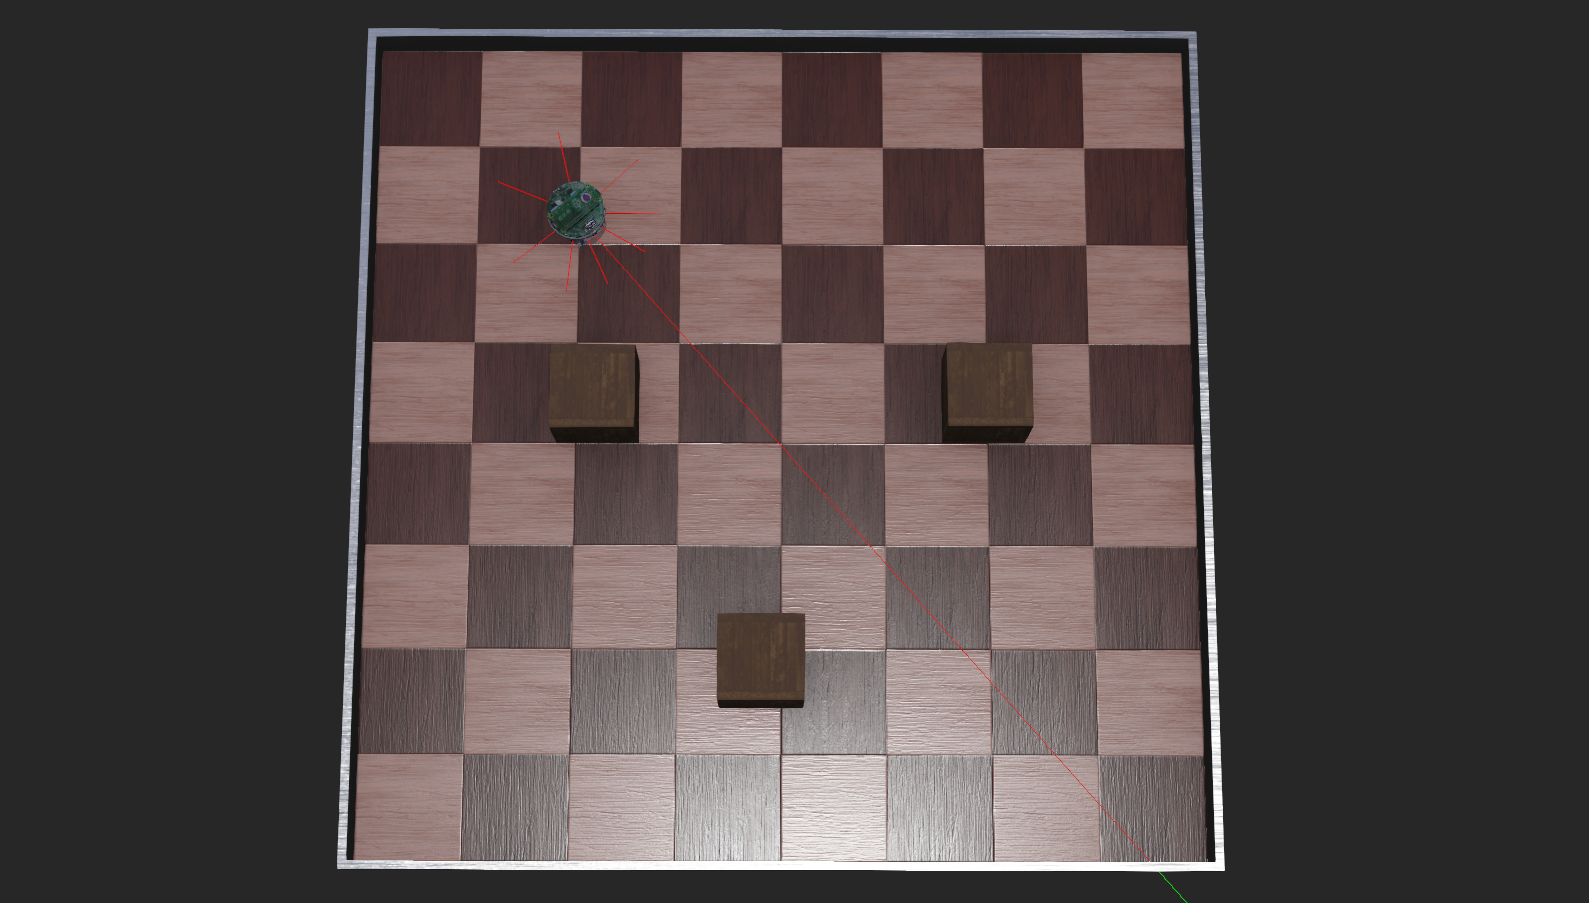
\includegraphics[width=\linewidth]{demos/figures/map_webots.png}
  \caption{Webots simulation with e-puck2}
  \label{fig:demos:mapping:map_webots}
\end{subfigure}
\begin{subfigure}{.95\textwidth}
  \centering
  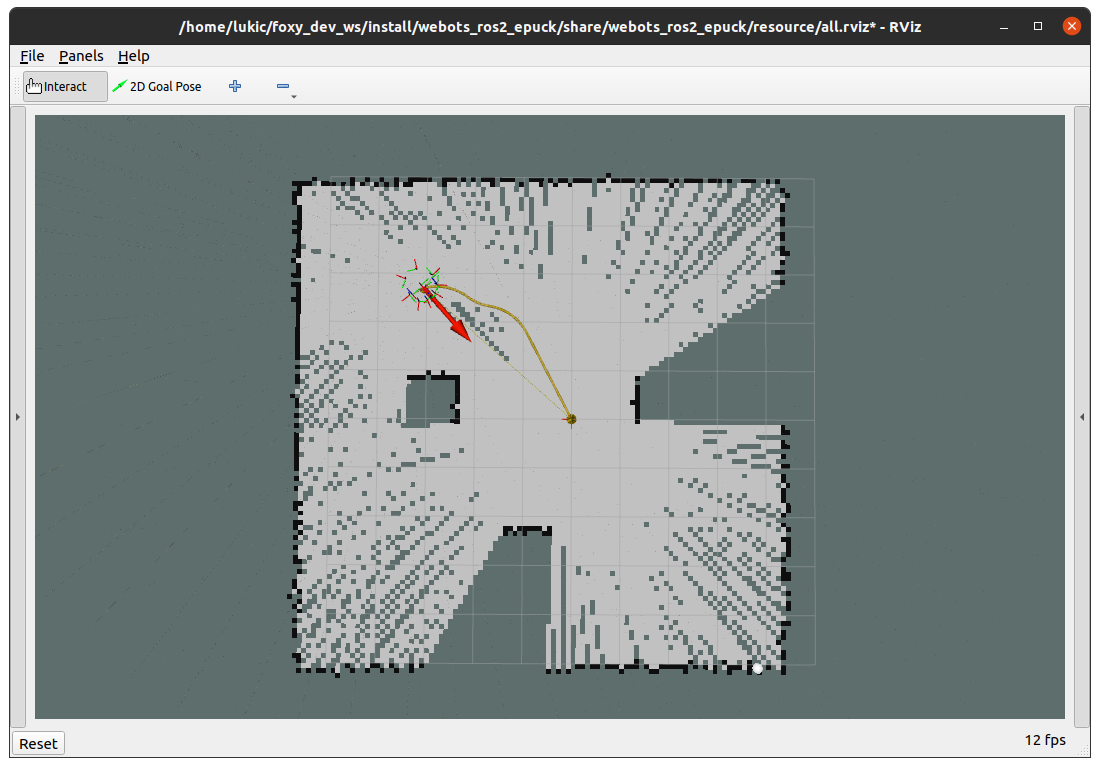
\includegraphics[width=\linewidth]{demos/figures/map_rviz.png}
  \caption{Map visualized in RViz2}
  \label{fig:demos:mapping:map_rviz}
\end{subfigure}
\caption{Mapping results shown in RViz2}
\label{fig:demos:mapping}
\end{figure}

Finally, the result can be observed in the figure above (Figure \ref{fig:demos:mapping}).

\section{Navigation Integration}
\label{sec:demos:navigation}

Another example is navigation.
For this demo, the Navigation2 community package is integrated.  
\begin{figure}[H]
    \centering
    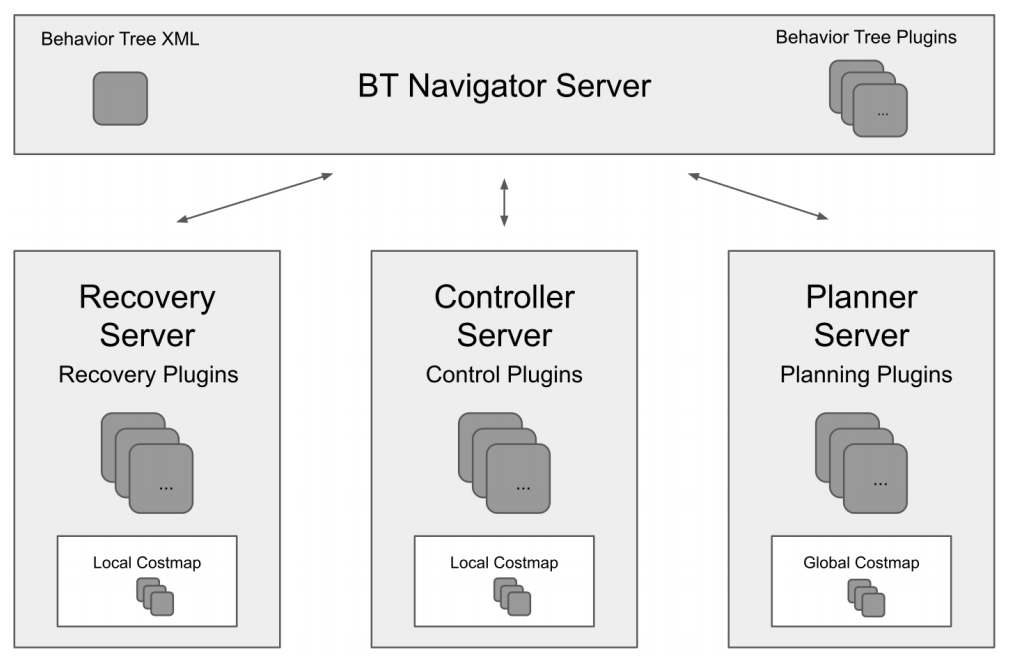
\includegraphics[width=\textwidth]{demos/figures/navigation_overview.png}
    \caption[Architecture of the Navigation2 package]{Architecture of the Navigation2 package\footnotemark}
    \label{fig:demos:navigation_overview}
\end{figure}
\footnotetext{The image is taken from official Navigation2 GitHub repository available at \url{https://github.com/ros-planning/navigation2}.}

% The package is extremely configurable, including hundreds of parameters.
% Therefore, it requires a good understanding of the background theoretical concepts to configure it efficiently \cite{zheng_ros_nodate}.

It uses transforms, maps, and measurements from range finders to control the robot's velocity, effectively avoiding obstacles and converging towards the destination (see Figure \ref{fig:demos:navigation_overview}).
Based on the provided map, it builds a global cost map used by a planner to find a global path (e.g., using an A star algorithm) to the destination.
Based on the data from the range finders, it builds a local cost map that is used by the controller server to avoid obstacles locally.
The controller server is also used to follow the path generated by the planner server, and it usually uses implementation called DWB local planner.
The planner considers the robot's maximum rotational and linear velocity and various critics (e.g., goal align and path align), to issue velocity commands \cite{macenski_marathon_2020-1}. 

% TODO: Add RViz2 screenshot
